\section{Esercitazione V.}

\begin{enumerate}

\item Studiare il condizionamento della funzione $f(x) = \cos(x)$. Fornire
esempi numerici che motivino i risultati ottenuti.

\begin{svol}
Studiare il condizionamento significa valutare se un problema è ben
condizionato, ovvero se a piccole perturbazioni sui dati corrispondono
errori dello stesso ordine.

Sia $x$ un dato, e $\tilde{x}$ lo stesso dato affetto da errore, $\Delta x =
\tilde{x}-x$.
\[
\textrm{Imponiamo } \Delta x = 10^{-13}, \textrm{ ovvero } 10^{-8} = \tilde{x} 
- x \Rightarrow \tilde{x} = 10^{-8} +x.
\]
Posto $y = \cos(x)$ e $\tilde{y} = \cos(\tilde{x})$, il problema è
trovare $\Delta y = \tilde{y} - y$. Dalla definizione e passando allo sviluppo
di Taylor si ha:
\[
\tilde{y} = f(x + \Delta x) = f(x) + f'(x)\Delta x + \cdots
\]
\[\tilde{y} - f(x) = f'(x)\Delta x + \cdots \]
da cui segue che $\Delta y = \tilde{y} - y \simeq f'(x)\Delta x$.

Tornando ai dati del problema si ha:
\[\Delta y = -\sin(x)\cdot 10^{-13}.\]
Poiché l'immagine della funzione $\sin$ è l'intervallo $[-1,1]$ possiamo
concludere che:
\[
\Delta y \subseteq [-1,1]\cdot 10^{-13} = [-10^{-8},10^{-8}].
\]
Da questo deduciamo che l'errore assoluto non cambia ordine di grandezza,
tuttavia noi vogliamo valutare l'errore relativo sui dati, ovvero trovare
$\frac{\Delta y}{y}$.

Valutiamo ora l'indice di condizionamento:
\[\frac{x}{\cos(x)}\cdot (-1)\sin(x) = -x \cdot \tan(x).\]
Da questo possiamo notare che, ad esempio in un intorno di $\frac{\pi}{2}$ 
l'indice di condizionamento ``esplode'' diventando $\simeq \infty$.

Vediamo quindi con Matlab il nostro caso:
\[
\frac{\Delta y}{y} = \frac{x}{f(x)}Df(x)\frac{\Delta x}{x} = 
\frac{\pi}{\cos(\pi)}(-1)\sin(\pi)\frac{10^{-8}}{\pi}.
\]
\begin{codice}
\begin{verbatim}
>> x = pi/2;
>> y = cos(x)

y =

     6.123233995736766e-17

>> 
>> deltax = 10^(-8);
>> 
>> xt = x - deltax;
>> yt = cos(xt)

yt =

     1.000000000045763e-08

\end{verbatim}
\end{codice}
Già il confronto tra questi due risultati ci dice che il divario tra le due 
soluzioni è eccessivamente elevato.
\begin{codice}
\begin{verbatim}
>> deltay = y-yt

deltay =

    -9.999999939225290e-09

>> deltay_ = -sin(x)*deltax

deltay_ =

    -1.000000000000000e-08

\end{verbatim}
\end{codice}
Qui sopra possiamo notare che, sia utilizzando la soluzione algebrica 
$\Delta y = y -\tilde{y}$ che quella analitica, l'ordine di grandezza
dell'errore relativo non cambia da quello di partenza sui dati.
\begin{codice}
\begin{verbatim}
>> % Calcolo dell'errore relativo sui dati.
>> erx = deltax/x;
>>
>> % Calcolo dell'indice di condizionamento cond.
>> cond = (x/cos(x))*(-sin(x));
>> 
>> % Errore relativo sui risultati.
>> ery = cond*erx

ery =

    -1.633123935319537e+08

>> 
\end{verbatim}
\end{codice}
L'ordine dell'errore relativo sui risultati è, in valore assoluto, di $10^8$,
molto più elevato di quello sui dati di partenza. Il problema è malcondizionato.
\end{svol}

\item Si approssimi il valore di $e^{-9}$, utilizzando lo sviluppo in serie
di $e^{x}$:
\[
e^x = 1 + x + \frac{x^2}{2!} + \frac{x^3}{3!} + \cdots 
\]
Quanti termini sono necessari per stabilizzare il risultato a $6$ cifre?

Ripetere il calcolo ricordando che è possibile scrivere $e^{-x} = \frac{1}{e^x}$.
Costruire, per un confronto, una tabella e un grafico degli errori relativi dei 
valori ottenuti sommando $n$ termini usando i due diversi algoritmi.

\begin{svol} Con due cicli \verb1while1 calcoliamo l'approssimazione di
$e^{-9}$ con una tolleranza \verb1t1 dell'ordine di $10^{-6}$, stampiamo quindi
il valore di \verb1i1 che rappresenta il numero di termini utilizzati.
\begin{codice}
\begin{verbatim}
>> format long
>> d = exp(-9);
>> x = -9;
>> a1 = 1 + x;
>> 
>> err = d-a1;
>> t = 10^-6;
>> i = 2;
>> 
>> while(abs(err)>t)
a1 = a1 + (x^i)/factorial(i);
err = d - a1;
i = i + 1;
end
>> i

i =

    34

>> a1

a1 =

     1.226613221354248e-04

>> d

d =

     1.234098040866796e-04

>> x = 9;
>> s = 1 + x;
>> a = 1/s;
>> err = d - a;
>> i = 2;
>> t = 10^-6;
>> while(abs(err)>t)
s = s + (x^i)/factorial(i);
a = 1/s;
err = d - a;
i = i + 1;
end;
>> i

i =

    18

>> a

a =

     1.240698022398142e-04

\end{verbatim}
\end{codice}
Il primo metodo impiega ben $34$ termini, mentre il secondo quasi la metà,
questo ci dice che la convergenza del primo è più lenta.

Calcoliamo ora due vettori contenenti le prime $34$ approssimazioni secondo
i due metodi e confrontiamole.
\begin{codice}
\begin{verbatim}
>> x = 9;
>> 
>> a1 = 1;
>> i = 2;
>> a1(2) = 1 - x;
>>
>> for i=3:35
a1(i) = a1(i-1) + ((-x)^(i-1))/factorial(i-1);
end
>> a1(35)

ans =

     1.236033868055714e-04

>> s = 1 + x;
>> a2 = 1;
>> a2(2) = 1/s;
>>
>> s(2) = 1 + x;
>> 
>> for i=3:35
s(i) = s(i-1) + (x^(i-1))/factorial(i-1);
a2(i) = 1/s(i);
end
>> a2(34)

ans =

     1.234098041059322e-04

>> d = exp(-9)

d =

     1.234098040866796e-04

>> ea1 = d - a1;
>> ea2 = d - a2;
>> er1 = ea1/d;
>> er2 = ea2/d;
>> 
>> [er1', er2']

ans =

   1.0e+06 *

  -0.008102083927575  -0.008102083927575
   0.064825671420603  -0.000809308392758
  -0.263349227646200  -0.000159457107477
   0.721175469554209  -0.000046110953067
  -1.494005099146711  -0.000017193845473
   2.493319924514945  -0.000007643750523
  -3.487667610977539  -0.000003836038004
   4.202173506084228  -0.000002087401582
  -4.448897750610261  -0.000001194654415
   4.202173506084228  -0.000000702393539
  -3.583790624940812  -0.000000416454028
   2.786543664079675  -0.000000245317013
  -1.991207052685690  -0.000000141847842
   1.316466520459563  -0.000000079739600
  -0.809895062276671  -0.000000043260166
   0.465921887365069  -0.000000022532170
  -0.251725146808410  -0.000000011230636
   0.128205635989315  -0.000000005348020
  -0.061759755409548  -0.000000002432304
   0.028223851042545  -0.000000001057070
  -0.012268771860897  -0.000000000439445
   0.005085209383436  -0.000000000174982
  -0.002014146580155  -0.000000000066832
   0.000763862275163  -0.000000000024520
  -0.000277891045581  -0.000000000008653
   0.000097140149887  -0.000000000002941
  -0.000032678340852  -0.000000000000964
   0.000010594489394  -0.000000000000305
  -0.000003314634614  -0.000000000000093
   0.000001001990078  -0.000000000000028
  -0.000000292997329  -0.000000000000008
   0.000000082966757  -0.000000000000002
  -0.000000022773142  -0.000000000000001
   0.000000006065012  -0.000000000000000
  -0.000000001568617  -0.000000000000000

>> n = linspace(1,35,35);
>> plot(n,er1,n,er2,'r');
>> 
\end{verbatim}
\end{codice}
Il primo metodo ha una convergenza molto più lenta, inoltre, come si può
vedere dal grafico, l'errore oscilla costantemente mentre nel secondo
questo fenomeno non si verifica.
\begin{figure}[!ht]\begin{center}
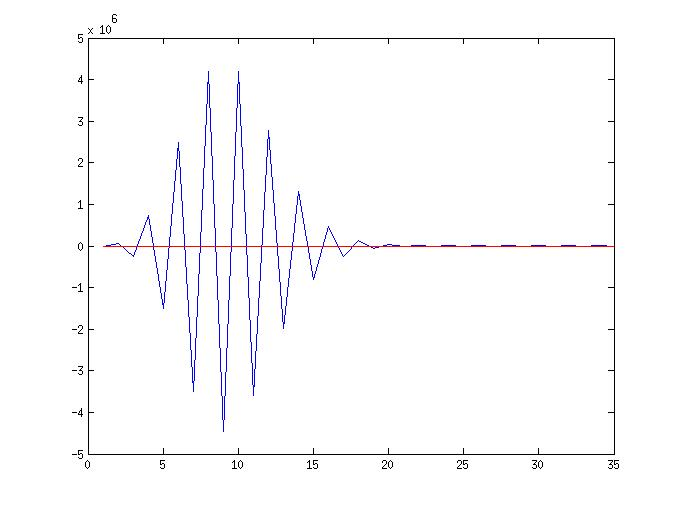
\includegraphics[scale=.50]{fig/es5-2.jpg}\end{center}
\caption{esercizio $2$.}
\end{figure}
\end{svol}

\item Siano $A = \text{hilb}(1000)$ e $B = \text{rand}(1000)$.
\begin{itemize}
\item[a)]Costruire il vettore $b$ in modo che il sistema $Ax = b$ sia risolto
da $x = \text{ones}(1000,1)$, e il vettore $c$ in modo che il sistema $By = c$
sia risolto da $y = \text{ones}(1000,1)$;
\item[b)]Calcolare i vettori $x$ e $y$ come soluzione dei sistemi lineari 
$Ax = b$ e $By = c$ utilizzando il comando \verb1\ (mldivide)1 di Matlab;
\item[c)]Calcolare gli errori relativi rapportandoli al numero di 
condizionamento delle corrispondenti matrici. Cosa si osserva?
\item[d)]Rappresentare in un grafico in scala semilogaritmica il condizionamento
della matrice di Hilbert di dimensioni variabili da $2 \times 2$ a $50 \times 
50$.
\end{itemize}

\begin{svol}Costruiamo le matrici come indicato.

\begin{codice}
\begin{verbatim}
>> H = hilb(1000);
>> B = rand(1000);
\end{verbatim}
\end{codice}

\begin{itemize}
\item[a)]
Calcoliamo i vettori $c$ e $b$ mediante prodotto riga per colonna delle
matrici e dei vettori costruiti, sfruttando la simmetria della relazione 
``$=$''.
\begin{codice}
\begin{verbatim}
>> x = ones(1000,1);
>> y = ones(1000,1);
>> 
>> b = A*x;
>> c = B*y;
\end{verbatim}
\end{codice}

\item[b)]Calcoliamo i vettori soluzione dei sistemi lineari di cui sopra
$x_1$ e $y_1$, per distinguerli da quelli iniziali.
\begin{codice}
\begin{verbatim}
>> x1 = A\b;
Warning: Matrix is close to singular or badly scaled.
         Results may be inaccurate. RCOND = 1.878903e-22. 
>> y1 = B\c;
>> 
\end{verbatim}
\end{codice}
Matlab già ora ci avverte che i risultati su $x_1$ potrebbero essere
affetti da errore.
\item[c)] Utilizziamo il comando \verb1cond()1 per calcolare l'indice di
condizionamento delle due matrici, calcoliamo quindi gli errori relativi
sulle soluzioni.
\begin{codice}
\begin{verbatim}
>> ca = cond(A)

ca =

   3.6665e+21

>> cb = cond(B)

cb =

   2.8027e+05

>> eax = x - x1;
>> eay = y - y1;
>> erx = erx./x;
>> ery = ery./y;
>> 
>> max(abs(erx))

ans =

   1.2879e+04

>> max(abs(ery))

ans =

   6.2221e-12

\end{verbatim}
\end{codice}
L'indice di condizionamento della matrice $A$ è molto elevato, infatti 
il massimo dell'errore relativo in modulo è molto più elevato di quello
calcolato per il vettore $y$ relativo alla matrice $B$, che ha infatti un 
indice di condizionamento molto minore.
\item[d)] Calcoliamo l'indice di condizionamento delle matrici di Hilbert
come richiesto e salviamole nel vettore \verb1CondH1. Utilizziamo quindi il
comando \verb1semilogy()1 che disegna il grafico in scala semilogaritmica
lungo l'asse delle $y$, utilizzando una scala lineare per l'asse delle $x$.
\begin{codice}
\begin{verbatim}
>> for i=2:50
CondH(i) = cond(hilb(i));
end
>> semilogy(CondH)
\end{verbatim}
\end{codice}
\begin{figure}[!ht]\begin{center}
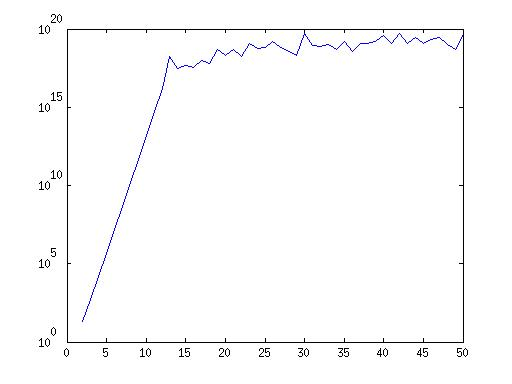
\includegraphics[scale=.50]{fig/es5-3.jpg}\end{center}
\caption{esercizio $3$.}
\end{figure}
\end{itemize}
\end{svol}

\item
Data la matrice $A$, e i vettori $b$, $x^*$ tali che:
\[
A = \left[ 
\begin{array}{cccc}
-4 & -1 & 1 & 1 \\
0 & -4 & -1 & 1 \\
-1 & -1 & 4 & 1 \\
1 & -1 & 0 & 4
\end{array}
\right], \quad 
b = \left[ 
\begin{array}{c}
-3  \\
-4 \\
3 \\
4
\end{array}
\right], \quad 
x^* = \left[ 
\begin{array}{c}
1  \\
1 \\
1 \\
1
\end{array}
\right];
\] 
preso un vettore $x^{(0)} \in \rr^{4}$ arbitrario, calcolare e tabulare al 
variare di $k = 0, \ldots, 10$, le seguenti quantità:
\[
\|x^*-x^{(k)}\|_1,\quad \|x^*-x^{(k)}\|_2,\quad \|x^*-x^{(k)}\|_\infty,
\]
dove
\[
x^{(k+1)} = (I-D^{-1}A)x^{(k)} + D^{-1}b, \quad k = 0, \ldots, 10.
\]
$I$ è la matrice identità e $D^{-1}$ è l'inversa della matrice diagonale $D$ 
estratta dalla matrice $A$. Mettere in un grafico la tabella costruita nella
prima parte dell'esercizio.

\begin{svol}
Iniziamo ad impostare i dati.
\begin{codice}
\begin{verbatim}
>> A = [-4 -1 1 1; 0 -4 -1 1; -1 -1 4 1; 1 -1 0 4]

A =

    -4    -1     1     1
     0    -4    -1     1
    -1    -1     4     1
     1    -1     0     4

>> b = [-3; -4; 3; 4];
>> x_ = ones(4,1);
>> 
>> D = diag(diag(A))

D =

    -4     0     0     0
     0    -4     0     0
     0     0     4     0
     0     0     0     4

>> I = eye(4);
>> Dinv = inv(D);
>>
>> x = rand(4,1);
\end{verbatim}
\end{codice}
Ora costruiamo la matrice contente i vettori $x^{(k+1)}$ e quella con
$x^*-x^{(k)}$.
\begin{codice}
\begin{verbatim}
>> for i=2:10
x(:,i) = (I-Dinv*A)*x(:,i-1) + Dinv*b;
end
>>
>> % le colonne di ex sono i vettori x-x^k
>> for i=1:10
ex(:,i) = x_ - x(:,i); 
end
\end{verbatim}
\end{codice}
Infine calcoliamo le tre norme per ogni $k$ richiesto e stampiamo la tabella
relativa.
\begin{codice}
\begin{verbatim}
>> for i=1:10
n1(i) = norm(ex(:,i));
n2(i) = norm(ex(:,i),2);
n1(i) = norm(ex(:,i),1);
ninf(i) = norm(ex(:,i),inf);
end
>> O = [linspace(1,10,10);n1;n2;ninf];
>> fprintf('\n k\t Norma 1 \t Norma 2 \t Norma Inf\n\n'),...
fprintf('%i \t %1.6f \t %1.6f \t %1.6f\n', O)

 k	 Norma 1 	 Norma 2 	 Norma Inf

1 	 2.444721 	 1.294401 	 0.902460
2 	 0.473086 	 0.262154 	 0.204245
3 	 0.185871 	 0.113172 	 0.101262
4 	 0.071560 	 0.043558 	 0.029724
5 	 0.022182 	 0.015684 	 0.014769
6 	 0.013994 	 0.008012 	 0.005531
7 	 0.005840 	 0.003309 	 0.002223
8 	 0.001676 	 0.001079 	 0.000921
9 	 0.001095 	 0.000568 	 0.000346
10 	 0.000443 	 0.000272 	 0.000191
>> 
\end{verbatim}
\end{codice}
\end{svol}

\end{enumerate}


\section{Esercitazione VI.}

\begin{enumerate}

\item
Determinare i coefficienti $a_i$ dei polinomi di grado $10$, $15$ e $20$ 
interpolanti la funzione $f(x) = e^x +1$ nei nodi equispaziati dell'intervallo
$[-1,1]$ (suggerimento: usare la matrice di Vandermonde e poi risolvere il
sistema lineare). Successivamente considerare i nuovi dati perturbati
$\tilde{f}(x_i) = f(x_i) + \varepsilon_i$ con $\varepsilon_i = (-1)^i10^{-5}$ e
calcolare i coefficienti $\tilde{a}_i$ del polinomio perturbato $\tilde{p}(x)$
interpolante i dati $(x_i, \tilde{f}(x_i))$. Confrontare i grafici dei due
polinomi.

Calcolare:
\[
\max |a_i - \tilde{a}_i| \quad \text{e} \quad \max |p(t)-\tilde{p}(t)|
\]
dove $t$ è un vettore formato da $101$ punti equispaziati in $[-1,1]$.

Ripetere l'esercizio usando i nodi di Chebishev:
\[x_i = \cos\left(\frac{(2i+1)\pi}{2n+2}\right), \quad i = 1,\ldots, n.\]
Commentare i risultati ottenuti.

\begin{svol}
Iniziamo con il calcolo dei tre grafici con punti equispaziati.
\begin{codice}
\begin{verbatim}
>> % Per avere polinomi di grado N occorrono N+1 punti.
>> x10 = linspace(-1,1,11);
>> x15 = linspace(-1,1,16);
>> x20 = linspace(-1,1,21);
>> 
>> % Costruzione delle matrici di Vandermonde.
>> V10 = vander(x10);
>> V15 = vander(x15);
>> V20 = vander(x20);
>> 
>> % Costruizione delle immagini della funzione.
>> b10 = exp(x10)+1;
>> b15 = exp(x15)+1;
>> b20 = exp(x20)+1;
>> 
>> % Calcolo dei coefficienti a dei polinomi.
>> a10 = V10\b10';
>> a15 = V15\b15';
>> a20 = V20\b20';
>> 
>> % Introduciamo i vettori delle perturbazioni
>> for i = 1 : 11
eps10(i) = ((-1)^i)*10^(-5);
end
>> for i = 1 : 16
eps15(i) = ((-1)^i)*10^(-5);
end
>> for i = 1 : 21
eps20(i) = ((-1)^i)*10^(-5);
end
>> 
>> % Calcolo delle immagini della funzione perturbate
>> b10_p = b10 + eps10;
>> b15_p = b15 + eps15;
>> b20_p = b20 + eps20;
>> 
>> % Calcolo dei coefficienti perturbati
>> a10_p = V10\b10_p';
>> a15_p = V15\b15_p';
>> a20_p = V20\b20_p';
>> 
>> % t è il vettore  di punti in cui valutare i polinomi.
>> t = linspace(-1,1,101);
>>
>> % Valutazione dei polinomi al variare di t.
>> y10 = polyval(a10, t);
>> y15 = polyval(a15, t);
>> y20 = polyval(a20, t);
>>
>> % Valutazione dei polinomi perturbati al variare di t.
>> y10_p = polyval(a10_p, t);
>> y15_p = polyval(a15_p, t);
>> y20_p = polyval(a20_p, t);
>>
>> % Stampa.
>> plot(t, y10, t, y10_p,'r');
>> plot(t, y15, t, y15_p,'r');
>> plot(t, y20, t, y20_p,'r');
>> 
\end{verbatim}
\end{codice}

Gli errori massimi sui coefficienti e sulle valutazioni dei polinomi
 sono i seguenti:
\begin{codice}
\begin{verbatim}
>> format long
>> % Calcolo degli errori.
>> E_coeff = [max(abs(a10-a10_p)) max(abs(a15-a15_p)) max(abs(a20-a20_p))]

E_coeff =

   1.0e+03 *

   0.000057870370372   0.011238023832376   2.568468176961571

>> E_y = [max(abs(y10-y10_p)) max(abs(y15-y15_p)) max(abs(y20-y20_p))]

E_y =

   0.000291264924889   0.005083726754011   0.106893964401543

>> 
\end{verbatim}
\end{codice}

Vediamo ora con i nodi di Chebishev come si comportano i nostri polinomi.
\begin{codice}
\begin{verbatim}
>> for i = 1 : 11
cheb10(i) = cos(((2*(i-1)+1)*pi)/(2*10+2));
end
>> for i = 1 : 16
cheb15(i) = cos(((2*(i-1)+1)*pi)/(2*15+2));
end
>> for i = 1 : 21
cheb20(i) = cos(((2*(i-1)+1)*pi)/(2*20+2));
end
>> 
>> for i = 1 : 21
cCheb20(i) = cos(((2*(i)+1)*pi)/(2*21+2));
end
>> 
>> 
>> V10_c = vander(cheb10);
>> V15_c = vander(cheb15);
>> V20_c = vander(cheb20);
>> 
>> b10_c = exp(cheb10)+1;
>> b15_c = exp(cheb15)+1;
>> b20_c = exp(cheb20)+1;
>> 
>> a10_c = V10_c\b10_c';
>> a15_c = V15_c\b15_c';
>> a20_c = V20_c\b20_c';
>> 
>> b10_cp = b10_c + eps10;
>> b15_cp = b15_c + eps15;
>> b20_cp = b20_c + eps20;
>> 
>> a10_cp = V10_c\b10_cp';
>> a15_cp = V15_c\b15_cp';
>> a20_cp = V20_c\b20_cp';
>> 
>> t = linspace(-1,1,101);
>> y10_c = polyval(a10_c,t);
>> y10_cp = polyval(a10_cp,t);
>> plot(t, y10_c, t, y10_cp,'r');
>> 
>> y15_c = polyval(a15_c,t);
>> y15_cp = polyval(a15_cp,t);
>> plot(t, y15_c, t, y15_cp,'r');
>> 
>> y20_c = polyval(a20_c,t);
>> y20_cp = polyval(a20_cp,t);
>> plot(t, y20_c, t, y20_cp,'r');
>> 
\end{verbatim}
\end{codice}


\begin{figure}[!ht]\begin{center}
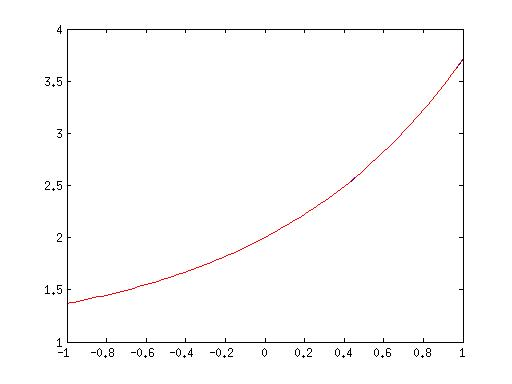
\includegraphics[scale=.35]{fig/es6-1a.jpg}
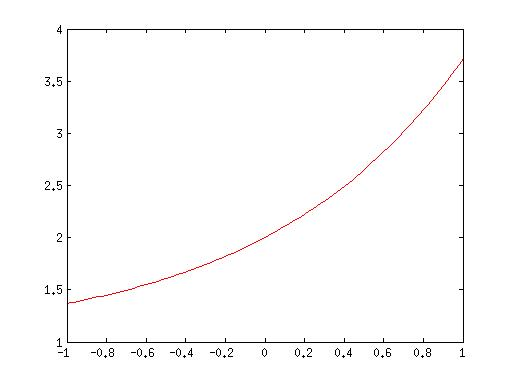
\includegraphics[scale=.35]{fig/es6-1d.jpg}
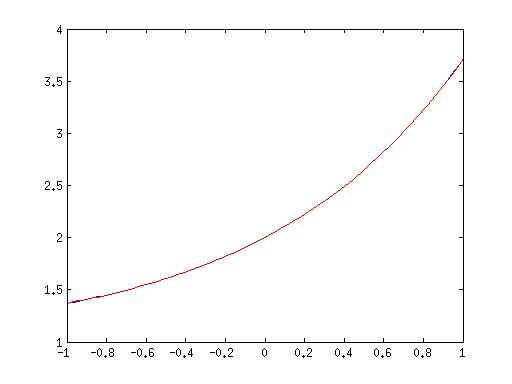
\includegraphics[scale=.35]{fig/es6-1b.jpg}
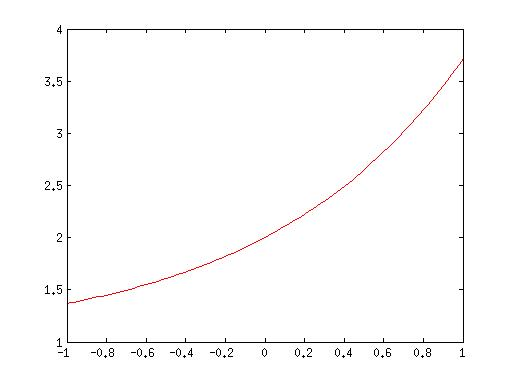
\includegraphics[scale=.35]{fig/es6-1e.jpg}
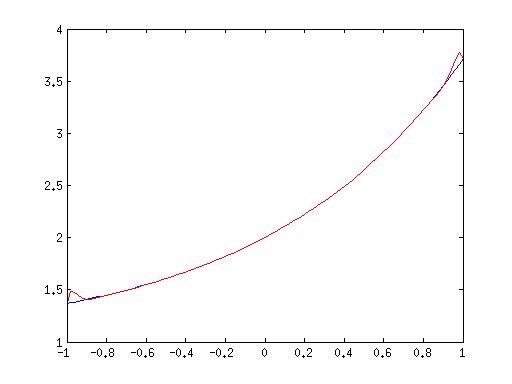
\includegraphics[scale=.35]{fig/es6-1c.jpg}
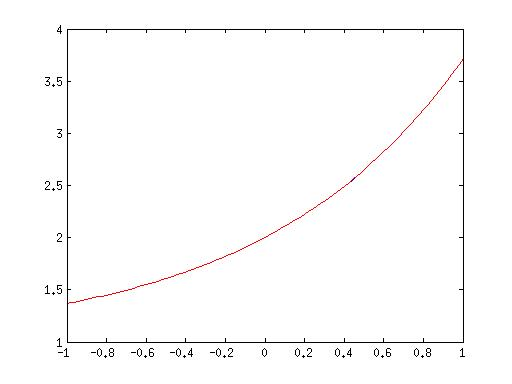
\includegraphics[scale=.35]{fig/es6-1f.jpg}
\end{center}
\caption{Sulla sinistra vediamo la curva calcolata con i nodi equispaziati,
sulla destra con i nodi di Chebishev.}
\end{figure}
Analizzando gli errori n modulo si ha:
\begin{codice}
\begin{verbatim}
> E_y = [max(abs(y10_c-y10_cp)) max(abs(y15_c-y15_cp)) max(abs(y20_c-y20_cp))]

E_y =

   1.0e-04 *

   0.248943037695071   0.272777793646206   0.290082490588262

>> E_coeff = [max(abs(a10_c-a10_cp)) max(abs(a15_c-a15_cp)) max(abs(a20_c-a20_cp))]

E_coeff =

   0.015792758827331   1.120696937190668  79.113672059826612

>> 
\end{verbatim}
\end{codice}

Dai grafici si può notare che all'aumentare del numero dei punti nel polinomio
interpolatore calcolato con nodi equispaziati l'errore aumenta (sopratutto
agli estremi), mentre con i nodi di Chebyshev questo fenomeno non si verifica.

Inoltre i grafici di sinistra hanno linee più distanti rispetto a quelli
di destra, purtroppo lo zoom non è sufficiente, però ad occhio si può notare,
oltre alla differenza agli estremi, che le curve di sinistra sembrano più
``spesse''. Questo perchè sono più distanti e quindi meno precise, come
l'analisi sugli errori ha evidenziato.
\end{svol}

\item Approssimare la radice quadrata di $x = 0.6$ considerando l'interpolazione
nella forma di Lagrange con nodi i tre quadrati perfetti $x_0 = 0.49$, 
$x_1 = 0.64$ e $x_2 = 0.81$. Stimare il resto di interpolazione e calcolare lo 
scarto rispetto al valore ottenuto con il comando \verb1sqrt1 di Matlab. 

Ripetere le operazioni aggiungendo il nodo $x = 0.36$.

\begin{svol}
Per stimare l'errore occorre calcolare la derivata terza nel caso dei
$3$ punti assegnati e quindi applicare il teorema dell'errore, o resto.
\[
|e(x)| = \frac{|f^{(n+1)}(\xi_x)|}{(n+1)!}|\omega_n(x)|
\leq \frac{M}{(n+1)!}|\omega_n(x)| \leq \frac{M}{(n+1)!}(b-a)^{n+1}.
\]

\[
|e(x)| \leq \frac{1}{6}\cdot\frac{3}{8\cdot\xi_x^{\frac{5}{2}}}\cdot(0.81-0.49)^{3}
\]

Per calcolare $\xi_x$ usiamo un vettore equispaziato tra $0.49$ e $0.81$.
\begin{codice}
\begin{verbatim}
>> x = [0.49 0.64 0.81];
>> y = sqrt(x);
>> 
>> p = polyfit(x,y,2);
>> 
>> polyval(p,0.6);
>> root = polyval(p,0.6)

root =

    0.7744

>> r = sqrt(0.6)

r =

    0.7746

>> err = abs(r-root)

err =

   1.8490e-04

>> vett = linspace(0.49,0.81);
>> M = max(abs(3./(8*sqrt(vett.^5))))

M =

    2.2312

>> ex = (M/6)*(0.81-0.49)^3

ex =

    0.0122
\end{verbatim}
\end{codice}
Come si può notare \verb1ex1 è un'approssimazione corretta (anche se poco 
precisa) dell'errore \verb1err1.

Ora vediamo cosa accade aggiungendo il dato come richiesto, analogamente per
il calcolo dell'errore prendiamo un $\xi_x$ compreso tra $0.36$ e $0.81$.
\begin{codice}
\begin{verbatim}
>> 
>> 
>> x1 = [0.36 0.49 0.64 0.81];
>> y1 = sqrt(x1);
>> 
>> p1 = polyfit(x1,y1,3);
>> 
>> root1 = polyval(p1,0.6)

root1 =

    0.7747

>> err1 = abs(r-root1)

err1 =

   6.3964e-05

>>
>> vett1 = linspace(0.36,0.81);
>> M1 = max(abs(-15./(16*sqrt(vett1.^7))))

M1 =

   33.4898

>> ex1 = (M1/6)*(0.81-0.36)^3

ex1 =

    0.5086

>> 

\end{verbatim}
\end{codice}
Aumentando la distanza tra due punti la precisione dell'approssimazione
dell'errore peggiora, come ci aspettavamo.
\end{svol}

\item
Disegnare sull'intervallo $[-1,1]$ il grafico della funzione $|\omega_n(x)|
= \prod_{i=0}^n(x-x_i)$ per alcuni valori di $n$ considerando nodi equispaziati.
Ripetere l'esercizio considerando i nodi di Chebyshev. Confrontare sullo
stesso sistema di riferimento i due grafici.

\begin{svol}
Iniziamo a definire queste due funzioni per costruire i nodi di Chebishev
e per calcolare la funzione $\omega_n$ dato un vettore di nodi.
\begin{codice}
\begin{verbatim}
function [x] = chebyshev(a,b,n)
%chebyshev calcola n nodi di chebyshev

for i=1:n
    x(i) = ((b-a)/2)*cos((2*i-1)*pi/(2*n+2)) + (a+b)/2; 
end

end


function [y] = omega_x(x, vec)
% omega_x := prod(x-x_i)

 n = length(x);
 y = zeros(n,1);
 for i = 1 : n
 y(i) = prod(x(i)-vec);
 end
 
end

\end{verbatim}
\end{codice}
A questo punto creiamo un vettore di dati e due vettori di nodi e vediamo
i risultati.
\begin{codice}
\begin{verbatim}
>> dati = linspace(-1,1,200);
>> 
>> nodi_e = linspace(-1,1,21);
>> nodi_c = chebyshev(-1,1,21);
>> 
>> y_e = omega_x(dati, nodi_e);
>> y_c = omega_x(dati, nodi_c);
>> 
>> plot(dati, y_e);
>> plot(dati, y_c);
>> 
>> plot(dati, y_e, dati, y_c, 'r');
>> 
\end{verbatim}
\end{codice}
\begin{figure}[!ht]\begin{center}
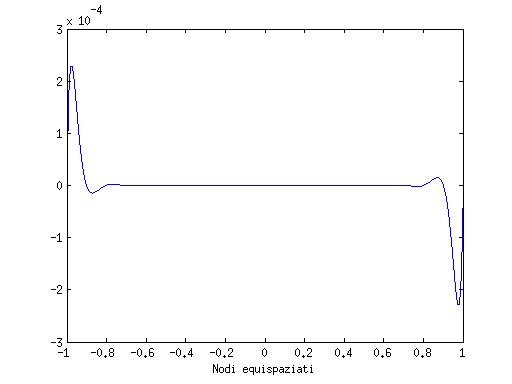
\includegraphics[scale=.35]{fig/es6-3a.jpg}
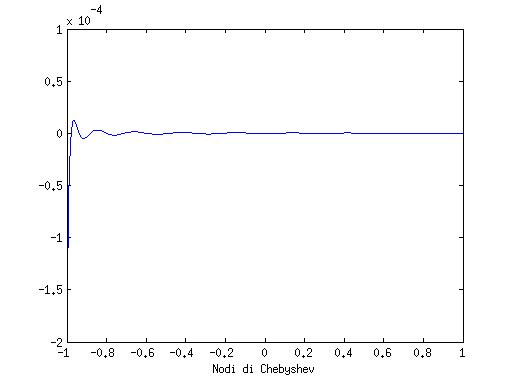
\includegraphics[scale=.35]{fig/es6-3b.jpg}
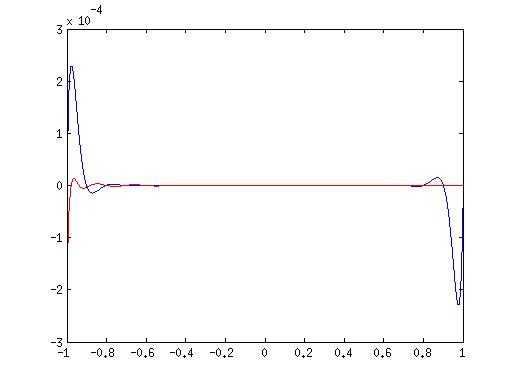
\includegraphics[scale=.35]{fig/es6-3c.jpg}
\end{center}
\end{figure}
\end{svol}

\end{enumerate}
